\documentclass[11pt, letterpaper]{article}

  \title{\LaTeX\ for Linguistics \\ (Unfinished December 2018 draft)}
  \author{Nicholas LaCara \\ University of Toronto}
  \date{}
  
    %% The geometry package manipulates page margins
    \usepackage{geometry}
    
    %% For denotation brackets
    \usepackage{stmaryrd}
      
    %% For LaTeX logos
    \usepackage{metalogo}
    
    %% For phonetic symbols and characters
    \usepackage{tipa}
    
    %% For in-document url formatting
    \usepackage{url}
    
    %% For drawing arrows
    \usepackage{pst-node}
    
    %% For drawing trees
    \usepackage{pst-jtree}
    
    %% For drawing trees with bracket notation
    \usepackage{tikz}
    \usepackage{tikz-qtree}
    
    %% For nice OT Tableaux
    \usepackage[open, medium, round]{OTtablx}
    
    %% For sequentially numbered examples
    \usepackage{gb4e}
    
    
  %% This is an example command I introduce later in the document.
  \newcommand{\highlight}[1]{\underline{\textbf{#1}}}

\begin{document}
  
  \maketitle
  
  \tableofcontents
  
  \newpage
%   \section{Introduction}
  
  \section{Background}
  
    \begin{itemize}
      \item \LaTeX\ (pronounced \textipa{["lA.tEx]} or \textipa{["lA.tEk]}, \textipa{["leI.tEk]}\ldots) is a popular system for typesetting technical documents in the fields of math, physics, engineering, and linguistics.
      
      \item It has native support for typesetting complex mathematical formulas:
      
	$$ i \hbar \frac{\partial}{\partial t}\vert\Psi(\mathbf{r},t)\rangle = \hat H\vert\Psi(\mathbf{r},t)\rangle $$
	
	\item Many of \LaTeX's features are useful for linguists and all academic and technical writers:
	
	  \begin{itemize}	    
	    \item Built-in sectioning and reference commands allow for easy structuring of documents and intra-document cross-references.
	    
	    \item The inbuilt math support is used for technical notation in all subfields.

	    \item The bibliography system (Bib\TeX) allows for easy citation management and outputs formatted reference sections.	    

	  \end{itemize}

      
      \item It has been expanded in various ways over the years to accommodate Linguistics, as well:
      
	  \begin{itemize}
	    
	    \item Extensions (known as packages) for drawing trees, tableaux, and other linguistic representations have been developed which allow for creating consistent, professional-looking diagrams and graphics.
	    
	    \item Other extensions allow for simple input of \textsc{ipa} characters
	  \end{itemize}
      
% 	\begin
    \end{itemize}
    
  
  \subsection{Why use \LaTeX?}
  
    \LaTeX\ is known to have a fairly steep learning curve, especially for those who are not used to coding or programming, though I think part of this reputation is undeserved.
    
      \begin{itemize}
	\item Unlike what-you-see-is-what-you-get word processors (\textsc{wysiwyg}; Microsoft Word, LibreOffice Write, and Google Docs), \LaTeX\ makes it difficult to format your documents in an arbitrary way.
	
	\item Things that are easy to do in Word are often hard to do 
	
	\item Part of the philosophy of using \LaTeX, however, is maintaining consistent formatting throughout a document. Thus, somethings are intentionally difficult to change.
	
	\item Many users coming from a \textsc{wysiwyg} background are not used to having so much control taken away from them.
	
      \end{itemize}

    \noindent \LaTeX\ has a number of technical features that 
  
      \begin{itemize}
	
	\item Built-in support for technical document structures and cross-referencing.
	
	\item Macros and custom commands allow for easy and consistent formatting throughout a document.
		
	\item Many linguistics-specific packages for typesetting and referencing examples, drawing trees, creating Optimality Theory tableaux
	
	\item Lack of formatting options, in principle, allows for focus on document structure.
	
      \end{itemize}
      
    \noindent Furthermore, it is free software (no cost, no commercial limitations).
    
      \begin{itemize}
	\item In principle, this means that it will be available in perpetuity for free.
	\item .tex files can be opened with any text editor on any computer.
        \item \LaTeX\ code will produce the same output no matter what system it is compiled on.
      \end{itemize}


  \subsection{What it's not}
  
    \begin{itemize}
      \item \LaTeX\ is a scripting language that instructs an interpretor on how to format documents.

      \item \LaTeX is not a word processor. 
      
    \end{itemize}

  \subsection{This document}
  
    \begin{itemize}
      \item The goal of this document is to provide novice and inexperienced users with a guide for using \LaTeX\ to create and typeset linguistics documents, though it is probably also of use to those outside of linguistics.
      
      \item The source code for this document has, as a result, been kept relatively simple and straightforward to make it easy to compare with the compiled document; only the minimal number of packages necessary have been used to create this document.
    \end{itemize}


  \section{Getting it}
  
  \subsection{MacOS}
  
    \begin{itemize}
      \item There are a couple of different ways of installing \LaTeX\ on MacOS.
      
      \item A simple way is to use the Mac\TeX\ distribution.
      
      \item Alternatively, one can use MacPorts to install \TeX live.
    \end{itemize}


  \subsection{Windows}
  
    \begin{itemize}
	\item Windows users can download and install MiK\TeX.
    \end{itemize}

  \subsection{Linux}
  
    \begin{itemize}
	\item Most popular \textsc{gnu}/Linux distributions (Ubuntu, Fedora, Linux Mint\ldots) include \LaTeX\ in their repositories. The following commands will install the full \LaTeX\ distribution (around 4ish \textsc{gb}):
	
	  \begin{itemize}
	  
	    \item Ubuntu: \verb+$ sudo apt-get install texlive-full+
	    \item Fedora: \verb+# yum install texlive-scheme-full+
	  
	  \end{itemize}
	  
    \end{itemize}
      
  \subsection{The internet}
  
    \begin{itemize}
      \item If you aren't ready to take the plunge, if you can't get the Mik\TeX\ installer to work, or if you just want to play around, there are websites that allow you to use \LaTeX\ online.
      
      \item Overleaf (\url{https://www.overleaf.com/}) allows for collaborative online editing of documents.
    \end{itemize}

      
  \section{Workflow}
  
  \subsection{Compiling a document}
  
    \begin{itemize}
    
	\item One of the main ways that using \LaTeX\ differs from using a word processor is the need to \emph{compile} a document. That is, it is necessary to convert the \LaTeX\ code into a human-readable .pdf file.
    
      \item There are different ways to compile a document, using different compilers. The compiler you need to use might depend on the packages you choose; most full \LaTeX\ installations will install all three following ones.
      
	  \begin{itemize}
	  
	    \item I raise this now since it raises compatibility issues for some packages that are useful for linguistics. 
	    
	    \item I'll point these compatibility issues out when they are relevant.
	  
	  \end{itemize}
      
      \item The “traditional” way is to send your document to the \LaTeX compiler. This creates a .dvi file that must be converted to a .ps file and then to a .pdf file.
      
	\begin{verbatim}
	  $ latex document.tex
	  $ dvips document.dvi
	  $ ps2pdf document.ps
	\end{verbatim}
	
	\item The script \verb+latexmk+ automates this process (see more below).
	

      \item However, pdf\LaTeX\ will produce a .pdf file directly. The resulting .pdf file is generally cleaner than th
      
	\begin{verbatim}
	  $ pdflatex document.tex
	\end{verbatim}
	
      \item Another option is \XeLaTeX, which will produce a .pdf directly, as well. \XeLaTeX\ provides several additional extensions to \LaTeX, including native \textsc{utf8} support and the ability to use all the fonts installed on your computer.
      
	\begin{verbatim}
	  $ xelatex document.tex
	\end{verbatim}
	

      \item Because of how the system interacts with external databases for things such as citations and document-internal references, you may need to compile the document more than once.
      
%       \item 
%       
    \end{itemize}
    
  \subsection{Compiling with Bib\TeX\ and other}
  
    \begin{itemize}
      \item One of the chief advantages to using \LaTeX\ is that it automates compiling bibliographies from in-line citations. This is usually done with a bibliography management system known as Bib\TeX\ (see Section \ref{S:Bib}).
      
      \item Because of the way this works, you will have to compile your document several times.
      
	  \begin{itemize}
	  
	    \item The first compilation identifies the citations in your document and creates a list of these citations to search for in a bibliography file (this list is stored in a .aux file).
	    
	    \item Running Bib\TeX\ will take the list of citations and search for them in the bibliography file, creating the references section for the document you are creating (which is stored in a .bbl file).
	    
	    \item Compiling the document a second time will integrate the contents of the .bbl file with your original document.
	    
	    \item Compiling the document a third time will link the in-line citations to the references that have been added to your document.
	  
	  \end{itemize}
	  
	\item This means that if you are using plain \LaTeX, you will have to use the following commands to produce a .pdf file if you change the citations in the document:
	
	\begin{verbatim}
	  $ latex document.tex
	  $ bibtex document.aux
	  $ latex document.tex
	  $ latex document.tex
	  $ dvips document.dvi
	  $ ps2pdf document.ps
	\end{verbatim}
	
	\item As noted above, the script \verb+latexmk+ automates this process, detecting changes to your .aux and .bbl files and running commands as necessary.
	
	\item Using a \LaTeX-specific editor can also automate this process.

    \end{itemize}


  \subsection{Using a \LaTeX-specific editor}
  
    \begin{itemize}
      \item 
    \end{itemize}

      
  \section{Basics of a \LaTeX\ document}
  
    \begin{itemize}
      \item A \LaTeX\ document is just a plain text document containing \LaTeX\ code.
      
      \item That code is processed by an interpreter that creates a formatted document from that plain text code.
    \end{itemize}

  
  \subsection{Preamble}
  
  \subsubsection{Document classes}
  
    \begin{itemize}
      \item The document class tells \LaTeX\ what kind of document you are creating. This can affect various commands made available to you.
      
      \item The document class must be declared at the beginning of your document with the \verb+documentclass+ command.
      
	\begin{exe}
	  \ex \verb!\documentclass[<options>]{<class>}! 
	\end{exe}

      
      \item For our purposes, the \verb+article+ class will be sufficient, but there are several other classes available, including \verb+book+, \verb+memoir+, and \verb+letter+.
      
      \item There are a number of options, which can be separated by commas:
      
	\begin{exe}
	  \ex \begin{tabular}[t]{ll}
	        \textit{Option}: 	& \textit{Function}: \\
% 	      \hline
	        \verb+10pt+ 		& Sets font size to 10pt \\
	        \verb+11pt+ 		& Sets font size to 11pt \\
	        \verb+12pt+ 		& Sets font size to 12pt \\
	        \verb+a4paper+		& Sets paper size to A4 \\
	        \verb+letterpaper+ 	& Sets paper size to US Letter \\
	        \verb+twoside+		& Sets different margins on even and odd pages \\
	      \end{tabular}

	\end{exe}

      \item To create an 11pt document on letter paper, start your document with the following command:
      
	\begin{exe}
	  \ex \verb!\documentclass[11pt, letterpaper]{article}! 
	\end{exe}

	
    \end{itemize}

  \subsubsection{Title, author, and date}
  
    \begin{itemize}
      \item You can declare the title of your document and the author with the \verb+\title+ and \verb+\author+ commands.
      
	\begin{exe}
	  \ex \verb+\title{\LaTeX\ for Linguists}+
	  \ex \verb+\author{Nicholas LaCara}+
	\end{exe}
	
      \item You'll if you want to include information like your affiliation, you can add that by including a line break with the \verb+\\+ command.
      
	\begin{exe}
	  \ex \verb+\author{Nicholas LaCara \\ University of Toronto}+
	\end{exe}
	
      However, there is no extra command for this.


      \item By default, the title will print the date that the document was compiled on. If you want to change that, you can use the \verb+\date+ command.
      
	\begin{exe}
	  \ex \verb+\date{Septembruary 35, 2068}+
	\end{exe}

      
    \end{itemize}

  
  \subsubsection{Packages}
  
    \begin{itemize}
      \item After you declare the document class and title information, you can call packages that you will use in the document.
      
      \item This is done with the \verb+\usepackage+ command.
      
	\begin{exe}
	  \ex \verb+\usepackage[<options>]{<package>}+
	\end{exe}

      \item I'll discuss specific packages in more detail in Section \ref{S:Packages}.
	
    \end{itemize}

  
  \subsubsection{Other things}
  
    \begin{itemize}
      \item One of the best things about \LaTeX\ is the ability to define custom commands, which helps simplify repetitive formatting tasks as well as create shortcuts for various.
      
      \item This should usually be done in the preamble before the start of the document, but after you call various packages you might want to use.
      
      \item This is done with the \verb+\newcommand+ command (or the \verb+\renewcommand+ command if a command needs to be redefined).
      
	\begin{exe}
	  \ex \verb+\newcommand{<command_name>}[no_of_arguments]{<definition>}+
	\end{exe}

      
      \item For instance, if you have to write the term `verb phrase ellipsis' many times, you might define a \verb+\VPE+ command that does most the work for you:
      
	\begin{exe}
	  \ex \verb+\newcommand{\VPE}{verb phrase ellipsis}+
	\end{exe}

      
      \item You can do more complicated things, too. For instance, if you want to create a command that \highlight{highlights text} so you can remember to come back and fix it later, you can define the following \verb+\highlight+ command:
      
	\begin{exe}
	  \ex \verb+\newcommand{\highlight}[1]{\underline{\textbf{#1}}}+
	\end{exe}

      	This basically says: Make a new command called \verb+\highlight+ that takes a single argument. Make the first argument bold and underline it.

      
    \end{itemize}

  
  \subsection{Body}
  
    \begin{itemize}
      \item You begin the body of your document with the \verb+\begin{document}+ command.
    \end{itemize}

  
  \subsubsection{The title}
  
    \begin{itemize}
      \item In order to typeset your title, use the \verb+\maketitle+ command.
      
      \item This will begin a new page and print the document titles, the author's name, and the date.
    \end{itemize}
  
  \subsubsection{Document structure and sections}\label{S:Structure}
  
    \begin{itemize}
      \item The \verb+article+ class includes the \verb+\part+, \verb+\section+, \verb+\subsection+, \verb+\subsubsection+, \verb+\paragraph+, and \verb+\subparagraph+ commands by default.
      
      \item These all have the same basic syntax: \verb+\section{<title>}+
      
      
      \item If you throw the \verb+\appendix+ command, all subsequent sections will be labeled with letters rather than numbers.
      
      \item These also all interact with \LaTeX's built-in cross-referencing system. Sectioning commands can be labeled and referred to in other places. This sentence is in Section \ref{S:Structure}.

      
	\begin{exe}
	  \ex\verb+\subsubsection{Document structure and sections}\label{S:Structure}+
	  \ex\verb+This sentence is in Section \ref{S:Structure}.+
	\end{exe}

      
      \item If you want to change the formatting of section headings, you can use a package like \verb+fancyhdr+.
    \end{itemize}

    
  \subsubsection{Bibliography}
  
    \begin{itemize}
      \item If you are using a bibliography (see Section \ref{S:Bib} below), you should put the bibliography at the end of the document.
      
      \item Assuming you are using an external bibliography for references, you can use this command to tell \textsc{Bib}TeX\ where that bibliography is: \verb+\+\verb+bibliography{<path_to_bib_file>}+
    \end{itemize}
    
  \subsubsection{Ending the document}
  
    \begin{itemize}
      \item When you reach the end of your document, you must call the \verb+\end{document}+ command.
      
      \item Any text after the \verb+\end{document}+ will be ignored.
    \end{itemize}


  
%   \subsection{A note on mathmode}

  \section{Native \LaTeX\ commands }
  
  \subsection{Text formatting}
  
    \begin{itemize}
      \item \verb+\textbf+ makes text bold.
      
      \item \verb+\textit+ makes text italic. However, you should generally use \verb+\emph+ for this purpose.
      
      \item \verb+\textsc+ sets text in small caps.
      
      \item \verb+\textsf+ sets text in sans serif.
      
      \item \verb+\texttt+ sets text in monospace.
      
      \item \verb+\underline+ underlines text (but it won't break across lines).
    \end{itemize}

  
  \subsection{Text size}
  
    The following are the standard sizes provided by the \verb+article+ class:\smallskip
  
    \begin{tabular}{ll}
      \verb+\tiny+ 		& {\tiny Call me Ishmael.} \\
      \verb+\scriptsize+ 	& {\scriptsize Call me Ishmael.} \\
      \verb+\footnotesize+	& {\footnotesize Call me Ishmael.} \\
      \verb+\small+: 		& {\small Call me Ishmael.} \\
      \verb+\normalsize+: 	& {\normalsize Call me Ishmael.} \\
      \verb+\large+: 		& {\large Call me Ishmael.} \\
      \verb+\Large+: 		& {\Large Call me Ishmael.} \\
      \verb+\LARGE+: 		& {\LARGE Call me Ishmael.} \\
      \verb+\huge+: 		& {\huge Call me Ishmael.} \\
      \verb+\Huge+:		& {\Huge Call me Ishmael.} \\
    \end{tabular}\medskip

    \noindent The syntax of these is a bit different from other \LaTeX\ commands. They can be used inside brackets:
    
      \begin{exe}
        \ex \verb+{\Large Call me Ishmael.}+
      \end{exe}
      
    \noindent Or, you can introduce them as an environment:
    
      \begin{exe}
        \ex \verb+\begin{Large} Call me Ishmael. \end{Large}+

      \end{exe}



  \subsection{Labeling and cross-references}
  
  \subsection{List environments}
  
  \subsection{Tables}
  
    \begin{itemize}
      \item To make a table, use the \verb+tabular+ environment.
    \end{itemize}

  
  \subsection{Footnotes}
  
    \begin{itemize}
      \item For most purposes, the \verb+\footnote+ command will do what you need. 
      
      \item Inserting a footnote into a document is easy.\footnote{Here is a footnote.}
      
	\begin{exe}
	  \ex \verb+Inserting a footnote into a document is easy.\footnote{Here is a footnote.}+
	\end{exe}
	
      \item There are a few places where putting footnotes will not work, like section titles.

    \end{itemize}

  
  \subsection{Changing fonts}\label{S:Fonts}
  
    \begin{itemize}
      \item The default font in \LaTeX\ is Computer Modern. It is instantly recognizable, but it has not aged well.
      
      \item Most \LaTeX\ distributions make available a large number of alternative fonts, however.
    \end{itemize}

  
  \section{Bibliography management and citations}\label{S:Bib}
  
    \begin{itemize}
      \item \LaTeX\ has some native capacity for in-text citations, but 
      
      \item Probably the most common package for bibliography and references is natbib.
    \end{itemize}

  \section{Packages}\label{S:Packages}
  
    \begin{itemize}
  
	\item Here I describe a number of useful packages, with an emphasis on those that are useful or important for linguistics.
	
	\item These packages extend \LaTeX's abilities by adding more commands. If you do not include the relevant packages in your preamble, these commands will not work and your document will not compile.
    
    \end{itemize}
  
  \subsection{Example packages}
  
    \begin{itemize}
      \item There are two or three packages that are in common use.
      
      \item All of them allow for automatic spacing of glosses in examples.
    \end{itemize}

  \subsubsection{linguex}
  
    \begin{itemize}
      \item Probably the most common example package, and the easiest to use.
    \end{itemize}

  
  \subsubsection{gb4e}
  
    \begin{itemize}
      \item gb4e is a bit more robust than linguex. It is the package that is being used in this document.
      
      \item It actually supports various kinds of syntax, including standard \LaTeX\ formatting for environments and commands.
      
	    \begin{verbatim}
	      \begin{exe}
	        \ex[*]{This is an example unglossed.}
	        \ex
	          \begin{xlist}
	            \ex[]{This is a subexample.}
	            \ex[]{\gll \'Este es un otro  ejemplo. \\
	                         this is a  other example \\
	                  \glt `This is another example.'}
	          \end{xlist}
	      \end{exe}
            \end{verbatim}

      \item However, Example formatting is not very flexible.
      
      \item It intentionally makes it so that superscripts and subscripts can be introduced with \textasciicircum\ and \_ outside mathmode. Some people like this feature, but it will screw up the placement of superscripts and subscripts in mathmode, which makes some formulas look bad. It also interferes with the code in many packages!
    \end{itemize}

  
  \subsubsection{expex}
  
    \begin{itemize}
      \item If you want total control over the formatting of your examples, \verb+expex+ can do just about anyting.
      
      \item However, it is the least intuitive and user friendly of the packages discussed here. It has it's own syntax that is notably different from standard \LaTeX\ syntax.
      
	\begin{verbatim}
	  \ex 
	    \ljudge* This is an example unglossed. 
	  \xe
	  \pex~
	    \a This is a subexample.
	    \a 
	      \begingl
	        \gla \'Este es un otro ejemplo. //
	        \glb This is a other example //
	        \glft `This is another example'//
	      \endgl
	  \xe
	\end{verbatim}

      
      \item It also introduces its own cross-referencing system, separate from the one built in to \LaTeX\ (though you can still use the built-in one).
    \end{itemize}

  
  \subsection{Trees}
  
    \begin{itemize}
      \item There are a lot of options in this domain, depending on your needs.
    \end{itemize}

  \subsubsection{qtree and variants}
  
    \begin{itemize}
      \item Qtree uses bracket notation to create trees. This makes it fairly straightforward to use.
      
      \item This syntax has recently been re-implemented with the TikZ drawing package using the \verb+tikz-qtree+ package.
      
	\begin{exe}
	  \ex 
	    \begin{verbatim}
  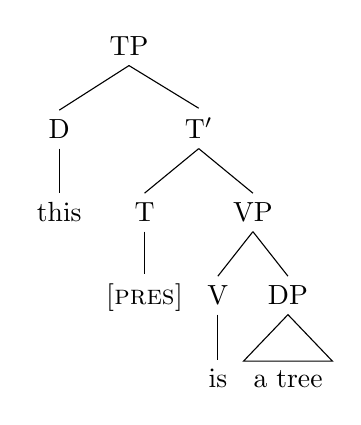
\begin{tikzpicture}
    \Tree [.TP [.D this ] [.T$'$ [.T \textsc{[pres]} ] % 
      [.VP [.V is ] [.DP \edge[roof]; {a tree} ] ] ] ]
  \end{tikzpicture}
	    \end{verbatim}


	  \ex 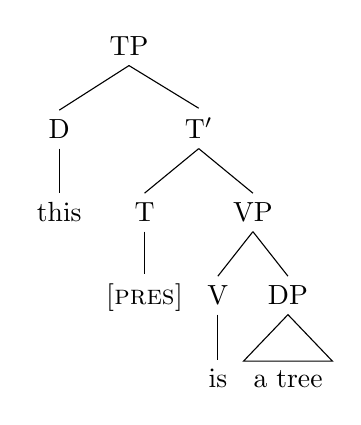
\begin{tikzpicture}
		\Tree [.TP [.D this ] [.T$'$ [.T \textsc{[pres]} ] % 
		  [.VP [.V is ] [.DP \edge[roof]; {a tree} ] ] ] ]
	      \end{tikzpicture}
   
	\end{exe}

      \item Many people swear by TikZ, though I find the bracket notation too cumbersome for more complicated trees. I also find the syntax for drawing a bit too unintuitive, but that's me.i
    \end{itemize}

  \subsubsection{pst-jtree}
  
    \begin{itemize}
       
      \item jTree is not very user-friendly, but it is very powerful and, with practice, will let you draw most anything.\footnote{It was created with producing multidominant trees in mind.}
            
	\begin{exe}
	  \ex
	    \begin{verbatim}
	\begin{jtree}
	  \! = {TP}
	    <left>[]{D}(<vert>[]{this})             ^<right>[]{T$'$}
	    <left>[]{T}(<vert>[]{\textsc{[pres]}})  ^<right>[]{VP}
	    <left>[]{V}(<vert>[]{is})               ^<right>[]{DP}
	    <vartri>[]{a tree}.
	  \end{jtree}
	    \end{verbatim}

	  \ex
	    \begin{jtree}
	      \! = {TP}
		<left>[]{D}(<vert>[]{this})		^<right>[]{T$'$}
		<left>[]{T}(<vert>[]{\textsc{[pres]}})	^<right>[]{VP}
		<left>[]{V}(<vert>[]{is})		^<right>[]{DP}
		<vartri>[]{a tree}.
	    \end{jtree}

	\end{exe}

      \item It allows (but sometimes requires) very fine-grained control how a tree appears.
	
      \item The big drawback to jTree is that it uses PSTricks for drawing, which is incompatible with pdf\LaTeX. You must use (plain) \LaTeX\ to compile documents that use jTree.
	
    \end{itemize}

      
  \subsection{Tableaux}
  
    \begin{itemize}
      \item It is possible to press \verb+tabular+ environments into service here, but it can be hard to do fancy (and important) stuff like draw dashed lines between unranked constraints.
      
	\begin{tabular}{|lll||c@{\ :\ }c|c|}
	  \hline
	    & & \textipa{/patak/} 	& \textsc{NoCoda}	& \textsc{Max}	& \textsc{Dep} \\
	  \hline\hline
	    a. & $\rightarrow$ & \textipa{pataka} & 		& 		& *	\\
	  \hline
	    b. & & \textipa{pata} 	& 			& *		& 	\\
	  \hline
	    c. & & \textipa{patak}	& *			& 		& 	\\
	  \hline
	\end{tabular}

      
      \item However, if you want professional looking tableaux, Nathan Sanders' \verb+OTtablx+ package creates excellent looking tableaux. You can even make complicated comparative tableaux:
      
	\begin{OTcomparative}{3}
	  \OTsolids{2}
	  \OTdashes{1}
	  \OTtoprow[\textipa{/patak/}]{\textsc{NoCoda}, \textsc{Max}, \textsc{Dep}}
	  \OTcandrow[\OThand]{pataka}{ 0, 0, 1}
	  \OTcandrow[]{pata}{ 0, \OTcompviol[W]{1}, \OTcompviol[L]{0}}
	  \OTcandrow[]{patak}{\OTcompviol[W]{1}, 0,\OTcompviol[L]{0} }
	\end{OTcomparative}

      \item As with jTree, mentioned above, \verb+OTtablx+ uses PSTricks, and so it cannot be used with pdf\LaTeX.
	
    \end{itemize}

  \subsection{Phonetic symbols}
  
    \begin{itemize}
      \item If you need to use \textsc{ipa} symbols in your document, the \verb+tipa+ package is absolutely excellent.
      
      \item The code \verb+\textipa{[f@"nE.RIks]}+ produces the following output: \textipa{[f@"nE.RIks]}

    \end{itemize}

  \subsection{Drawing}

    \begin{itemize}
    
      \item I use the \verb+pst-node+ package from PSTricks for drawing arrows between things.
      
	\begin{exe}
	  \ex[*]{\rnode{wh}{Who$_i$} did Bill meet Sally [$_{Adjunct}$ before he talked to \rnode{trace}{$t_i$}]?}
	    \ncbar[angle=-90, linearc=0.25ex, linestyle=dashed, nodesep=2pt]{->}{trace}{wh}\ncput*{*}
	\end{exe}
	
      \item As mentioned above, you can also use \verb+tikz+ to draw.

    \end{itemize}

  
  \subsection{Semantic formulas}
  
    \begin{itemize}
      \item \LaTeX's native mathmode provides a lot of functionality for typesetting semantic formulas and denotations. A few extra packages are occasionally necessary for 
      
      \item The package \verb+stmaryrd+ provides standard denotation brackets $\llbracket.\rrbracket$
      
      \item The packages \verb+amssymb+ and \verb+amsmath+ also provide additional functionality
      
    \end{itemize}
    
    \begin{exe}
    \ex\begin{verbatim}
	  $\llbracket\mbox{the}\rrbracket = \lambda P. \lambda Q. \exists x. %
      [Q(x) \wedge \forall y. [P(y) \rightarrow x = y]]$
       \end{verbatim}

    \ex[]{$\llbracket\mbox{the}\rrbracket = \lambda P. \lambda Q. \exists x. %
      [Q(x) \wedge \forall y. [P(y) \rightarrow x = y]]$}
    \end{exe}


  
  \subsection{Non-English languages and scripts}
  
    \begin{itemize}
      \item Owing to its age, \LaTeX's support for non-Latin scripts is not particularly good. 
      
	\begin{itemize}
	
	  \item \LaTeX\ was first released in 1983. Unicode would not come into existence until the late 80s.
	  
	  \item {[NOTE ABOUT FONT SUPPORT]} Additionally, most modern font formats (like TrueType and OpenType) had not been invented yet.
	  
	  \item For various technical reasons, there are different econdings for typefaces. 
	
	\end{itemize}
      
      \item If you want to diacritics or accent marks on Latin characters, there is fairly good native support for this if you are willing to use \LaTeX's built-in commands.
      
      \item If you want to type in characters directly, you must use the package \verb+inpuntenc+, with the \verb+utf8+ option:
      
	\begin{verbatim}
	  \usepackage[utf8]{inputenc}
	\end{verbatim}

	If you don't do this, nothing will appear if you type a character like \texttt{\"{o}} .
	
      \item If you want to change various section headings, dates, hyphenation rules, and other language-specific parts of the document, use the \verb+babel+ package:
      
	\begin{verbatim}
	  \usepackage[<language>]{babel}
	\end{verbatim}

      \item However, if you want/need to use non-Latin characters, you should really consider using \XeLaTeX! \XeLaTeX\ supports modern \textsc{utf8} encoding natively and works with your system fonts.
    \end{itemize}
    
  \subsection{Fonts and typographical stuff}
  
    \begin{itemize}
      \item There are a number of fonts and typefaces that come with the full installation of \LaTeX; the Danish \TeX\ User Group keeps a pretty good list at \url{http://www.tug.dk/FontCatalogue/}.
      
      \item If you want to use Times both in regular text and in mathmode, use either the package \verb+mathptmx+ or the packages \verb+newtxtext+ and \verb+newtxmath+ together.

    \end{itemize}

    
%   \subsubsection{What if I don't want to use \XeLaTeX?}
%     
%     \begin{itemize}
% 	
%       \item Some scripts, like Cyrillic have fairly good support through the \verb+T2+ encoding. You can load this with the \verb+fontenc+ package:
%       
% 	\begin{verbatim}
% 	  \usepackage[T2]{fontenc}
% 	\end{verbatim}
% 
%       \item Even then, if you want to use non-Latin characters, things become even more difficult.
%       
% 	\begin{itemize}
% 	
% 	  \item Chinese, Japanese, and Korean have historically been supported in \LaTeX\ through the \verb+CJK+ package. Getting this to work is not known to be easy.\footnote{A lot of this boils down to getting and installing the right sorts of fonts. It is doable, but not very straightforward.}
% 	  
% 	  \item Arabic script and Hebrew are also supported
% 
% 	
% 	\end{itemize}
%       
%       \item 
% 	
%     \end{itemize}
    
  \subsection{Graphics and images}
  
    \begin{itemize}
      \item Another place that \LaTeX\ shows its age is in how it handles graphics, and this is probably one of the places it is most frustrating to use.
      
      \item \LaTeX\ has no native support for graphics. Graphics and images must be imported with the \verb+graphicx+ package.
      
      \item The frustrating thing is that the graphics formats you can use in a document are different depending on which method you use to compile your document.
      
	\begin{itemize}
	
	  \item latex $\rightarrow$ dvips $\rightarrow$ ps2pdf \\	  
	    You can import postscript graphics (.eps files), and nothing else. If you want to use graphics with this mode, you must convert them to .eps files first.
	    
	  \item pdflatex \\
	    You can import jpeg, pdf, and png files, amongst others. It can also use .eps file (but secretly converts them to .pdf format).
	    
	  \item xelatex \\
	    \XeLaTeX\ supports most graphics formats. 
	
	\end{itemize}
      
      \item The reason this leads to frustration is that you might need to use a specific compiler for other reasons. For instance, if you use \verb+pstricks+ for drawing trees, you won't be able to use pdf\LaTeX.%\footnote{\XeLaTeX\ allows one to use \verb+pstricks+ as well as several graphics formats.}
	
	
      \item If you need to import and manipulate .pdf documents, the \verb+pdfpages+ is extremely useful.
    \end{itemize}

  \section{Slides and posters with Beamer}
  
    \begin{itemize}
      \item You can use \LaTeX\ to create presentation slides and posters using the Beamer document class.\footnote{The name \emph{beamer} comes from the German loanword for a projector.}
      
%       \item 
    \end{itemize}

  \subsection{Presentations with Beamer}
  
    \begin{itemize}
      \item Beamer is designed to create presentation slides (\emph{frames} in its terms).
      
      \item Beamer includes special commands for creating and laying out slides, controlling the flow of information.
      
      \item Each slide is defined in a frame environment, which contains standard \LaTeX\ code:
      
	\begin{verbatim}
	  \begin{frame}{This is the title of the slide}
	    The following list will appear after a pause:\pause
	      \begin{itemize}
	        \item This is the first item.
	        \item This is the second item.
	      \end{itemize}
	  \end{frame}
	\end{verbatim}

      \item The output is .pdf file that can be viewed in any .pdf viewer.
	
    \end{itemize}

  
  \subsection{Make a real handout with the \texttt{beamerhandout} package}
  
    \begin{itemize}
      \item Printing out your slides 6-up is for PowerPoint users. The \verb+beamerhandout+ package makes it easy to convert your slides into a true handout!
    \end{itemize}

  \subsection{Posters using \texttt{beamerposter}}
  
    \begin{itemize}
      \item The \verb+beamerposter+ package makes one huge Beamer frame to be used as a poster.
    \end{itemize}

  
  \section{Additional resources}
  
    \begin{itemize}
      \item The \LaTeX\ Wikibook is a good, free resource: \url{https://en.wikibooks.org/wiki/LaTeX/}
      
	\begin{itemize}
	
	  \item The chapter on Linguistics has more examples and some different package examples.
	
	\end{itemize}
      
      \item The ShareLaTeX documentation at \url{https://www.sharelatex.com/learn/Main_Page} is very comprehensive! 
      
      \item When things fail, check out StackExchange!
    \end{itemize}


\end{document}
